\chapter{Zárógondolat}\label{sect:Ending}
A Cloud RAN új környezetében tehát lehetőség van arra, hogy az üzemeltetők nagyobb hálózati kapacitást és lefedettséget biztosíthassanak az előfizetőik számára kisebb összköltség (total cost of ownership, TCO) mellett, lsd. \figref{cool}-es ábra. Nyilván felmerül a kérdés, hogy vajon mikor kerül sor a Cloud RAN ipari léptékű megvalósítására? Kétségtelen, hogy a Cloud-RAN skálázhatósága páratlan lehetőségeket rejt magában. Továbbá a felhő alapú infrastruktúra tervezéséhez és általános elterjedéséhez szükséges gazdasági elemzések a CAPEX/OPEX (beruházási és működtetési költségek) oldaláról közelítenek, azokat minél jobban redukálni próbálják. Az energiafogyasztó fizikális elemek (pl. air conditioning) számának csökkentésével és a központosítással viszont várható ezen költségek csökkenése. A ZTE és China Mobile is végzett számításokat a C-RAN struktúrák energiamegtakarításának területén: hasonló eredménnyel 67-80 \% körüli megtakarítást számoltak a BBU Pool-ban, a hagyományos RAN architektúrákhoz viszonyítva. Érdekes információ például, hogy a C-RAN rendszereknél a CAPEX költségek megközelítően 80\%-át csak a RAN teszi ki, így ennek csökkentésében rendkívüli a potenciál. \cite{GreenCRAN}
A fent említtetek alapján a Cloud RAN alapja lehet a jövő szélessávú mobilhálózatainak. A mobil hálózati architektúra forradalma a közelgő virtualizációval várható, hiszen általános cél, hogy ne kézzel fogható, gyakran kusza kábelrendszerrel (vagy legalábbis, minél kevesebbel) kelljen megvalósítani a hálózati architektúrákat. A felhő alapú rendszerek megannyi új szolgáltatásnak és új alkalmazásnak lehet az alapja. A szolgáltatók a folyamatos fejlődés útján bizonyára nyitni fognak a Cloud RAN koncepció irányába.
\begin{figure}[!ht]
\centering
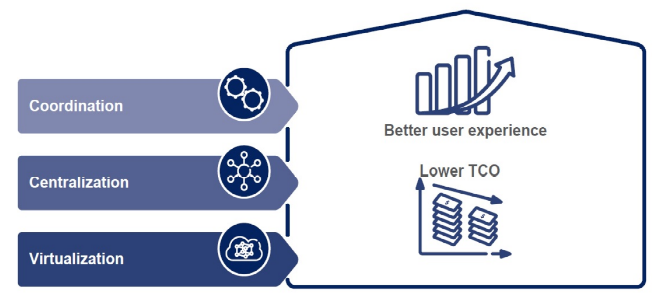
\includegraphics[width=0.7\textwidth, keepaspectratio]{figures/cool.png}
\caption{A Cloud-RAN eszköszök és előnyök} 
\label{fig:cool}
\end{figure}
%----------------------------------------------------------------------------
